\documentclass{oblivoir}
\usepackage{graphicx} % Required for inserting images
\usepackage{verbatim}

\usepackage[a4paper, total={7in, 9in}]{geometry}
\setcounter{tocdepth}{5}
\setcounter{secnumdepth}{5}
\hypersetup{
    colorlinks=true,
    linkcolor=blue
}

\title{HW4}
\author{C311054 박민서}
\date{2025년 5월 24일}

\begin{document}

\maketitle

\section{N-Queen problem}

\subsection{LISP 문법}
\paragraph*{length}
리스트의 길이를 반환하는 함수
\begin{verbatim}
(length '(2 3 1)) -> 3
\end{verbatim}

\paragraph*{nth}
리스트의 n번째 원소를 반환하는 함수
\begin{verbatim}
(nth 1 '(3 4 1 2)) -> 4
\end{verbatim}
첫번째 원소는 0번임에 주의한다.

\paragraph*{NIL}
LISP에서 false는 NIL로 표현한다.

\paragraph*{abs}
절댓값을 반환하는 함수
\begin{verbatim}
(abs -2) -> 2
\end{verbatim}

\paragraph*{progn}
여러 코드를 묶어서 실행할 수 있게 해준다.
반환값은 마지막 표현식의 결과이다.
\begin{verbatim}
>> (progn (print "Hello") (print "World"))
Hello 
World
\end{verbatim}

\subsection{작동 방식}
nqueen과 check이라는 두 개의 재귀함수와 nqueen의 초기 호출로 구성된다.
LISP에도 반복문이 있긴하지만 재귀함수가 함수형 언어에 더 적합한 방법이라고 생각해서 재귀함수로 구현하였다.

\subsubsection{nqueen함수 정의}

\begin{verbatim}
(DEFUN nqueen (li row col)  ;1
   (COND 
     ((> row 4) (print li)) ;2
     ((> col 4) NIL)        ;3
     (T (COND               ;4
          ((check (cons col li) 1) (progn   ;5
                                     (nqueen (cons col li) (+ row 1) 1) ;6
                                     (nqueen li row (+ col 1))          ;7
                                   )
          )
          (T (nqueen li row (+ col 1)))     ;9
        )
     )
   )
)
\end{verbatim}
주석에 적은 줄 번호별로 설명하겠다.

\paragraph*{1}nqueen이라는 함수는 인자로 리스트, 행번호, 열번호를 받는다.
row-major로 체스판의 모든 위치를 순회하면서 row행 col열에 퀸을 놓을지 결정하는 함수이다.
li의 n번째 원소에 n행에 배치된 퀸의 열번호를 저장한다. li가 (1 4 3 2)라면 1행 1열, 2행 4열, 3행 3열, 4행 2열에 퀸을 배치했다는 의미이다. (이는 이해를 돕기 위한 설명으로, 뒤에서 설명하겠지만 실제로는 순서가 역순으로 들어간다.)

\paragraph*{2}만약 행번호가 4를 초과했다면 4행까지 퀸을 성공적으로 배치했다는 뜻이므로 완성된 리스트를 출력한다.

\paragraph*{3}열번호가 4를 초과했다면 탐색중인 행에서 퀸을 배치할 열을 1열부터 4열까지 검사해봤지만 모두 실패했다는, 즉 해당 행에는 퀸을 놓을 수 있는 곳이 없다는 뜻이므로 NIL을 반환한다.

\paragraph*{4}두번째 COND는 굳이 따로 분기하지 않아도 되지만 재귀함수의 종료조건과 구분하기 위해 이중으로 사용했다.

\paragraph*{5}check함수에게 해당 행,열에 퀸을 배치한 리스트와 검사를 시작할 인덱스인 1을 넘겨준다. cons는 원소를 리스트의 맨 앞에 붙이기 때문에 리스트에서는 1행의 퀸의 열번호가 마지막이 되고 리스트의 앞으로 올수록 더 높은 행번호에 대한 값이다. 
맨 앞에 삽입한 원소에 대해 기존의 값들과 충돌이 없는지를 확인하는 것이 check이다. 따라서 탐색을 시작할 인덱스로 1을 넘겨주는 것이다. 0번째 인덱스와 1부터 마지막 인덱스의 값들을 비교한다.

\paragraph*{6}check에서 T를 반환했다면 배치가능하다는 의미이므로 그대로 배치된 리스트, 다음 행번호, 열번호는 1부터 다시 시작하는 nqueen을 호출한다.

\paragraph*{7,9}모든 경우의 수를 찾기 위해 check에서 퀸 배치에 성공했든 실패했든 다음 열에 대한 nqueen을 수행한다. 

\subsubsection{check함수 정의}
\begin{verbatim}
(DEFUN check (li i)     ;1
       (COND
         ((>= i (length li)) T)     ;2
         (T (COND       ;3
              ((= (car li) (nth i li)) NIL)             ;4
              ((= (abs (- (car li) (nth i li))) i) NIL) ;5
              (T (check li (+ i 1)))                    ;6
            )
         )
       )
)
\end{verbatim}
\paragraph*{1}
검사할 리스트와 탐색 시작 지점의 인덱스 i를 파라미터로 갖는다.

\paragraph*{2}
탐색 지점의 인덱스가 리스트 길이보다 크거나 같으면 리스트 범위를 초과하는 것이다. 
이 조건에 해당하는 경우는 1행에 대한 검사 중이어서 li에 원소가 1개일 때이거나 li의 마지막 원소까지 무사히 검사를 마친 경우이다. 따라서 맨 앞에 삽입된 원소가 그 자리에 배치가능하다는 뜻의 T를 반환해준다.

\paragraph*{3}
여기서도 종료조건과의 구분을 위해 분기하였다.

\paragraph*{4}
첫번째 배치 불가능 케이스이다. 앞선 행들에 이미 배치되어 있는 퀸들과 열번호가 같으면 안된다. 따라서 맨 앞의 원소와 i번째 원소값이 같다면 NIL을 반환한다.

\paragraph*{5}
두번째 불가능 케이스는 같은 대각선 상에 위치하는 경우이다. 같은 대각선 상에 위치한다는 것은 행번호의 차이와 열번호의 차이가 같다는 것으로 판별할 수 있다. 맨 앞 원소의 열번호에서 i번째 원소의 열번호를 빼고 절댓값을 취한다. 이 값과 i값을 비교하는데, 맨 앞 원소는 0번째 인덱스이므로 i-0, 즉 i가 곧 행번호의 차이기 때문이다. 

이렇게 같은 열에 위치하는 경우와 같은 대각선에 위치하는 경우를 걸러내었다. 마지막으로 같은 행에 위치하는 경우가 남았는데 이는 nqueen에서 row-major로 순회하면서 한 행에서 하나씩만 퀸을 배치하기 때문에 check에서 처리하지 않아도 된다.

\paragraph*{6}
이렇게 한 인덱스에서 충돌 조건을 모두 통과하였다면 다음 인덱스로 넘어가 판별을 반복한다.

\subsubsection{nqueen 실행}
\begin{verbatim}
(nqueen '() 1 1)
\end{verbatim}
이제 함수를 실행하기만 하면 된다.
초기값으로 빈 리스트와 순회를 시작할 위치 1행 1열을 넣는다.

\subsection{실행 결과}
\begin{figure}[h]
    \centering
    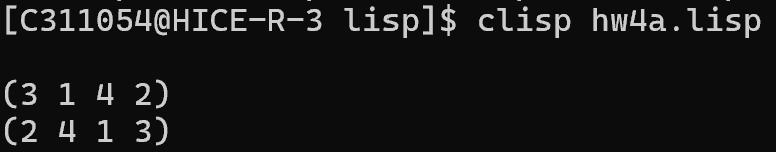
\includegraphics[width=0.5\linewidth]{hw4a.png}
    \caption{hw4a.lisp}
    \label{fig:fig1}
\end{figure}

리스트에 열번호가 역순으로 들어가 있으니 다시 뒤집어서 출력해야되는게 아닐까싶지만 배치 가능한 케이스의 체스판을 위아래 반전한 경우도 또다른 배치 가능 케이스가 되기 때문에 상관없다.

\section{Insertion Sort}
\subsection{LISP 문법}
\paragraph*{append}
리스트 여러 개를 이어서 하나의 리스트로 반환하는 함수
\begin{verbatim}
(append '(3 2) '() '(1)) -> '(3 2 1)
\end{verbatim}

\paragraph*{subseq}
(subseq li start end)의 형태로 li의 start부터 end-1까지를 반환하는 함수
\begin{verbatim}
(subseq '(4 2 5 1) 1 4) -> '(2 5 1)
\end{verbatim}

\subsection{작동 방식}
\subsubsection{insertion\_sort함수 정의}
\begin{verbatim}
(DEFUN insertion_sort (li1 li2) ;1
       (print (append li1 li2)) ;2
       (COND
         ((> (length li2) 0) (insertion_sort (insert li1 (- (length li1) 1) (car li2)) (cdr li2))) ;3
         (T NIL)    ;4
       )
)
\end{verbatim}
\paragraph*{1}
insertion\_sort함수는 삽입을 할 타겟 원소를 골라서 insert함수에게 전해주는 역할을 한다.
li1은 타겟원소의 앞부분, 즉 정렬되어 있는 부분이다.
li2는 뒷부분으로 여기에서 맨 앞 원소를 하나씩 빼서 li1에 삽입하는 식으로 정렬이 이루어진다.

\paragraph*{2}
원소 하나가 정렬될 때마다, 즉 이 함수가 한번 실행될 때마다 li1와 li2를 합친 전체 리스트를 출력한다.

\paragraph*{3}
insert함수에는 삽입이 이루어질 리스트(li1), 그 리스트의 마지막 인덱스, 삽입할 원소를 인자로 넘긴다.
삽입이 완료된 li1와 맨 앞 원소를 제거한 li2를 인자로 하여 다시 insertion\_sort를 실행한다.

\paragraph*{4}
이 함수의 종료조건은 li2의 길이가 0이 됐을 때이다.

\subsubsection{insert함수 정의}
\begin{verbatim}
(DEFUN insert (li i a) ;1
        (COND
          ((= i -1) (cons a li))                    ;2
          ((> (nth i li) a) (insert li (- i 1) a))  ;3
          ((<= (nth i li) a) (append                ;4
                               (subseq li 0 (+ i 1))    ;5
                               (list a)                 ;6
                               (COND                    
                                 ((= i (- (length li) 1)) '())          ;7
                                 (T (subseq li (+ i 1) (length li)))    ;8
                               )
                             )
          )
        )
)
\end{verbatim}

\paragraph*{1}
삽입이 진행되는 리스트 li, 삽입할 원소와 비교하는 원소의 인덱스 i, 삽입할 원소인 a를 파라미터로 받는다.

\paragraph*{2}
i는 가장 끝에서 부터 앞으로 한칸씩 이동하는데 만약 -1까지 왔다면 리스트의 모든 원소보다 a가 작다는 뜻이므로 리스트의 맨 앞에 삽입해야 한다. 이는 cons로 쉽게 처리할 수 있다.

\paragraph*{3}
i번째 인덱스의 값보다 a가 크다면 i를 앞으로 한 칸 이동하여 다시 insert를 실행한다.

\paragraph*{4}
i번째 인덱스의 값보다 a가 작거나 같다면 i의 바로 뒷자리에 a를 삽입한다.
이는 인덱스 i를 기준으로 li를 둘로 쪼개고 사이에 a를 넣어 합친 리스트를 반환하는식으로 동작한다.

\paragraph*{5}
0부터 i번째 인덱스까지의 리스트

\paragraph*{6}
append의 인자로 쓰기 위해 리스트로 만든 a

\paragraph*{7}
만약 i가 마지막 인덱스였다면 뒷부분은 빈 리스트가 된다.

\paragraph*{8}
그 외의 경우에는 i+1부터 마지막원소까지의 리스트를 뒤에 붙여준다.

\subsubsection{insertion\_sort 실행}
\begin{verbatim}
(princ "TC1:")
(insertion_sort '() '(11 33 23 45 13 25 8 135))
(terpri)
(princ "TC2:")
(insertion_sort '() '(83 72 65 54 47 33 29 11))
\end{verbatim}
앞서 말했듯 insertion\_sort는 li2에서 원소를 빼 li1에 삽입하는 식으로 정렬이 진행된다. 따라서 초기값으로 li1에는 빈 리스트, li2에는 정렬할 리스트를 넣어줘야 한다.

\subsection{실행 결과}
\begin{figure}[h]
    \centering
    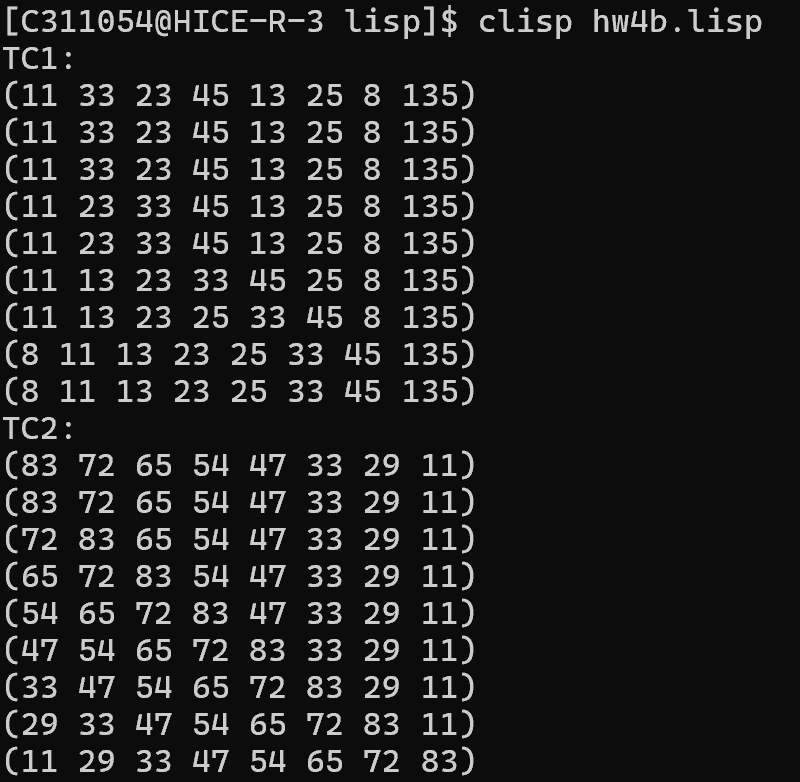
\includegraphics[width=0.5\linewidth]{hw4b.png}
    \caption{hw4b.lisp}
    \label{fig:fig2}
\end{figure}
첫번째 줄은 초기 리스트이고 다음줄부터 첫번째 원소를 정렬한 결과, 두번째 원소를 정렬한 결과...그리고 마지막 줄이 마지막 원소를 정렬한 결과이자 모든 원소에 대한 정렬이 완료된 리스트이다.

\end{document}
